\documentclass[../mn-notatki.tex]{subfiles}

\begin{document}

\section{Interpolacja wielomianowa funkcji}

\subsection{Definicje}
\begin{tcolorbox}
Niech dane będą
\begin{itemize}
    \item $x_0 < x_1 < \ldots < x_n \in \mathbb{R}$ \textbf{(węzły interpolacji)}
    \item $y_0 < y_1 < \ldots < y_n \in \mathbb{R}$ \textbf{(wartości)}
    \item $\mathcal{F}$ ustalona klasa funkcji $f \in \mathcal{F} \rightarrow
    \mathbb{R}$.
\end{itemize}
Problem wyznaczenia funkcji $f \in \mathcal{F}$ spełniającej warunki
\[
f(x_i) = y_i, \tab \text{dla } i = 0, 1, \ldots, n
\]
nazywamy \textbf{zadaniem interpolacji}.
\end{tcolorbox}

\subsection{Wzór interpolacyjny Newtona}
\begin{tcolorbox}
\[
p_n(x) = \sum_{k=0}^{n} a_k \prod_{j=0}^{k-1} (x-x_j)
\]
\[
a_k = \frac{y_k - p_{k-1}(x_k)}{\prod_{j=0}^{k-1}(x_k - x_j)}
\]
\end{tcolorbox}

\begin{itemize}
    \item \textbf{Dodanie kolejnych punktów nie narusza współczynników już
    policzonych.}
    \item Zmiena kolejności węzłów \textbf{zmienia} postać wzoru Newtona.
    \item Zmiana wartości $y_0$ wymaga przeliczenia wszystkiego od początku.
    \item \textbf{Nie należy przekształcać wielomianu}, lecz wyznaczyć wartość
    $p_n(x)$ stosując \textbf{wzór Hornera}.
    \item W praktyce współczynniki wyznacza się stosując \textbf{metodę ilorazów
    różnicowych}.
\end{itemize}

\subsection{Wzór interpolacyjny Lagrange'a}
\begin{tcolorbox}
\[
p(x) = \sum_{k=0}^{n} y_k L_k(x)
\]
\[
L_k(x) = \prod_{\substack{j=0\\j\neq k}}^{n} \frac{x-x_i}{x_k-x_j}
\]
\end{tcolorbox}

\begin{itemize}
    \item Nie należy przekształcać wielomianu Lagrange'a do postaci kanonicznej.
    Obliczenia wartości pośrednich dokonujemy ewaluując odpowiednie wielomiany
    $L_k$.
    \item Dla ustalonyh węzłów $x_i$ wielomiany $L_j$ są stałe, zmiana
    kolejności węzłów też ich nie zmienia.
    \item Interpolacja Lagrange'a jest zwłaszcza przydatna gdy \textbf{węzły
    się nie zmieniają}, a zmieniają się tylko wartości.
\end{itemize}

\subsection{Ilorazy różnicowe}

\begin{tcolorbox}
\[
f[x_0] = f(x_0)
\]
\[
f[x_0,x_1] = \frac{f(x_1) - f(x_0)}{x_1 - x_0}
\]
\[
f[x_0,\ldots, x_k] = \frac{f[x_1, \ldots, x_k] - f[x_0, \ldots, x_{k-1}]}{x_k - x_0}
\]
\end{tcolorbox}

\subsection{Metoda Newtona z ilorazami różnicowymi}

\begin{tcolorbox}
\[
p_n(x) = \sum_{k=0}^{n} f[x_0,\ldots,x_k] \prod_{i=0}^{k-1} (x-x_i)
\]
\end{tcolorbox}

\begin{center}
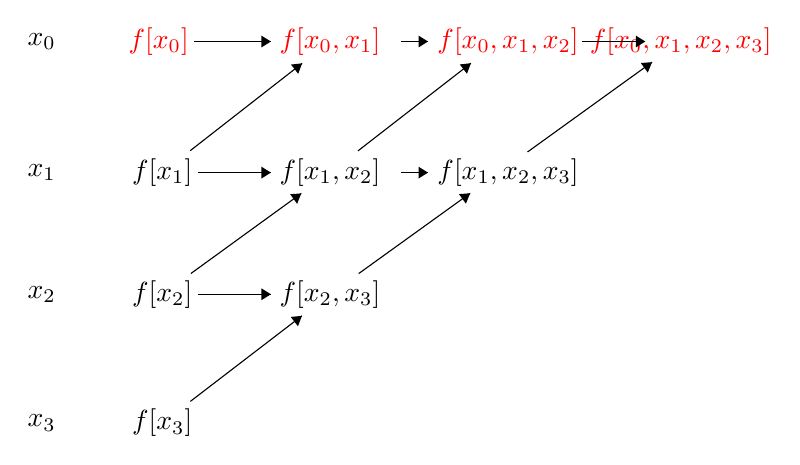
\begin{tikzpicture}[scale=0.15]
\tikzstyle{every node}+=[inner sep=0pt]
% \draw [black] (10.7,-17.4) circle (3);
\draw [red] (10.7,-17.4) node {$f[x_0]$};
% \draw [black] (25.2,-17.4) circle (3);
\draw [red] (25.2,-17.4) node {$f[x_0,x_1]$};
% \draw [black] (39.5,-17.4) circle (3);
\draw [red] (39.5,-17.4) node {~~$f[x_0,x_1,x_2]$};
% \draw [black] (54.9,-17.4) circle (3);
\draw [red] (54.9,-17.4) node {\tab\tab$f[x_0,x_1,x_2,x_3]$};
% \draw [black] (11,-28.5) circle (3);
\draw (11,-28.5) node {$f[x_1]$};
% \draw [black] (11,-38.8) circle (3);
\draw (11,-38.8) node {$f[x_2]$};
% \draw [black] (11,-49.7) circle (3);
\draw (11,-49.7) node {$f[x_3]$};
% \draw [black] (25.2,-28.5) circle (3);
\draw (25.2,-28.5) node {$f[x_1,x_2]$};
% \draw [black] (25.2,-38.8) circle (3);
\draw (25.2,-38.8) node {$f[x_2,x_3]$};
% \draw [black] (39.5,-28.5) circle (3);
\draw (39.5,-28.5) node {~~$f[x_1,x_2,x_3]$};
% \draw [black] (0.8,-17.4) circle (3);
\draw (0.8,-17.4) node {$x_0$};
% \draw [black] (0.8,-28.5) circle (3);
\draw (0.8,-28.5) node {$x_1$};
% \draw [black] (0.8,-38.8) circle (3);
\draw (0.8,-38.8) node {$x_2$};
% \draw [black] (0.8,-49.7) circle (3);
\draw (0.8,-49.7) node {$x_3$};
\draw [black] (13.7,-17.4) -- (20.2,-17.4);
\fill [black] (20.2,-17.4) -- (19.4,-16.9) -- (19.4,-17.9);
\draw [black] (31.2,-17.4) -- (33.5,-17.4);
\fill [black] (33.5,-17.4) -- (32.7,-16.9) -- (32.7,-17.9);
\draw [black] (46.5,-17.4) -- (51.9,-17.4);
\fill [black] (51.9,-17.4) -- (51.1,-16.9) -- (51.1,-17.9);
\draw [black] (13.36,-26.65) -- (22.84,-19.25);
\fill [black] (22.84,-19.25) -- (21.9,-19.35) -- (22.51,-20.13);
\draw [black] (14,-28.5) -- (20.2,-28.5);
\fill [black] (20.2,-28.5) -- (19.4,-28) -- (19.4,-29);
\draw [black] (13.43,-37.04) -- (22.77,-30.26);
\fill [black] (22.77,-30.26) -- (21.83,-30.33) -- (22.42,-31.14);
\draw [black] (14,-38.8) -- (20.2,-38.8);
\fill [black] (20.2,-38.8) -- (19.4,-38.3) -- (19.4,-39.3);
\draw [black] (13.38,-47.87) -- (22.82,-40.63);
\fill [black] (22.82,-40.63) -- (21.88,-40.72) -- (22.49,-41.51);
\draw [black] (27.57,-26.66) -- (37.13,-19.24);
\fill [black] (37.13,-19.24) -- (36.19,-19.34) -- (36.8,-20.13);
\draw [black] (31.2,-28.5) -- (33.5,-28.5);
\fill [black] (33.5,-28.5) -- (32.7,-28) -- (32.7,-29);
\draw [black] (27.63,-37.05) -- (37.07,-30.25);
\fill [black] (37.07,-30.25) -- (36.12,-30.32) -- (36.71,-31.13);
\draw [black] (41.93,-26.75) -- (52.47,-19.15);
\fill [black] (52.47,-19.15) -- (51.52,-19.22) -- (52.11,-20.03);
\end{tikzpicture}
\end{center}
% {"nodes":[{"x":107,"y":174,"text":"f[x_0]","isAcceptState":false},{"x":252,"y":174,"text":"f[x_0,x_1]","isAcceptState":false},{"x":395,"y":174,"text":"f[x_0,x_1,x_2]","isAcceptState":false},{"x":549,"y":174,"text":"f[x_0,x_1,x_2,x_3]","isAcceptState":false},{"x":110,"y":285,"text":"f[x_1]","isAcceptState":false},{"x":110,"y":388,"text":"f[x_2]","isAcceptState":false},{"x":110,"y":497,"text":"f[x_3]","isAcceptState":false},{"x":252,"y":285,"text":"f[x_1,x_2]","isAcceptState":false},{"x":252,"y":388,"text":"f[x_2,x_3]","isAcceptState":false},{"x":395,"y":285,"text":"f[x_1,x_2,x_3]","isAcceptState":false},{"x":8,"y":174,"text":"x_0","isAcceptState":false},{"x":8,"y":285,"text":"x_1","isAcceptState":false},{"x":8,"y":388,"text":"x_2","isAcceptState":false},{"x":8,"y":497,"text":"x_3","isAcceptState":false}],"links":[{"type":"Link","nodeA":0,"nodeB":1,"text":"","lineAngleAdjust":0,"parallelPart":0.5,"perpendicularPart":0},{"type":"Link","nodeA":1,"nodeB":2,"text":"","lineAngleAdjust":0,"parallelPart":0.5,"perpendicularPart":0},{"type":"Link","nodeA":2,"nodeB":3,"text":"","lineAngleAdjust":0,"parallelPart":0.5,"perpendicularPart":0},{"type":"Link","nodeA":4,"nodeB":1,"text":"","lineAngleAdjust":0,"parallelPart":0.5,"perpendicularPart":0},{"type":"Link","nodeA":4,"nodeB":7,"text":"","lineAngleAdjust":0,"parallelPart":0.5,"perpendicularPart":0},{"type":"Link","nodeA":5,"nodeB":7,"text":"","lineAngleAdjust":0,"parallelPart":0.5,"perpendicularPart":0},{"type":"Link","nodeA":5,"nodeB":8,"text":"","lineAngleAdjust":0,"parallelPart":0.5,"perpendicularPart":0},{"type":"Link","nodeA":6,"nodeB":8,"text":"","lineAngleAdjust":0,"parallelPart":0.5,"perpendicularPart":0},{"type":"Link","nodeA":7,"nodeB":2,"text":"","lineAngleAdjust":0,"parallelPart":0.5,"perpendicularPart":0},{"type":"Link","nodeA":7,"nodeB":9,"text":"","lineAngleAdjust":0,"parallelPart":0.5,"perpendicularPart":0},{"type":"Link","nodeA":8,"nodeB":9,"text":"","lineAngleAdjust":0,"parallelPart":0.5,"perpendicularPart":0},{"type":"Link","nodeA":9,"nodeB":3,"text":"","lineAngleAdjust":0,"parallelPart":0.5,"perpendicularPart":0}]}

% \subsection{Zjawisko Runge'go}
% \subsection{Zbieżność wielomianów iterpolacyjnych}

% \subsection{Wielomiany Czybyszewa}
% Aby zmniejszyć błąd można odpowiednio dobrać punkty \textit{(węzły)}.

% % \begin{tcolorbox}
% \textbf{Wielomiany Czybyszewa I rodzaju}

% \begin{table}[!htb]
%     \begin{minipage}{.5\linewidth}
%         \[
%         T_0(x) = 1 \tab T_1(x) = x
%         \]
%         \[
%         T_n(x) = 2x \cdot T_{n-1}(x) - T_{n-2}(x)
%         \]
%     \end{minipage}%
%     \begin{minipage}{.5\linewidth}
%         \begin{gather*}
%         T_2(x) = 2x^2 - 1\\
%         T_3(x) = 4x^2 - 3x\\
%         T_4(x) = 8x^4 - 8x^2 +1
%         \end{gather*}
%     \end{minipage}%
% \end{table}

% \end{tcolorbox}

\subsection{Błąd interpolacji wielomianowej}
\begin{tcolorbox}
Jeżeli $f i\in \mathcal{C}^{n+1}[a,b], p \in \Pi_n$ interpoluje $f$ w punktach
$x_0, x_1, \ldots, x_n \in [a,b]$ to dla każdego $x \in [a,b]$ istnieje
$\xi_x \in (a,b)$ takie, że
\[
f(x) - p(x) = \frac{f^{(n+1)}(\xi_x)}{(n+1)!} \prod_{i=0}^{n} (x-x_i)
\]
\end{tcolorbox}

\subsubsection{Przykład}

Jaki jest błąd przybliżenia $f(x) = \sin(x)$ wielomianem interpolacyjnym
stopnia $9$ w przedziale $[0,1]$?

\[
|\sin(x) - p_9(x)| \leqslant
\left| \frac{\sin^{(10)}(\xi_x)}{10!} \prod_{j=0}^{9} (x-x_i) \right|
\leqslant \frac{1}{10!} \approx 2.8 \cdot 10^{-7}
\]

\pagebreak
\subsection{Interpolacja Hermite'a}

\begin{tcolorbox}
\[
p_n(x) = \sum_{k=0}^{n} f[x_0,\ldots,x_k] \prod_{i=0}^{k-1} (x-x_i)
\]
\end{tcolorbox}

\subsubsection{Uogólnienie ilorazów różnicowych}

\begin{tcolorbox}
\[
f[x_0,\ldots,x_k] = \begin{cases}
\frac{f^{(k)}(x_0)}{k!} \tab\tab\tab \text{~jeżeli } x_0 = x_k\\
\frac{f[x_1,\ldots,x_k] - f[x_0,\ldots,x_{k-1}]}{x_k - x_0}
\tab \text{jeżeli } x_0 \neq x_k
\end{cases}
\]
\end{tcolorbox}

% \pagebreak
\end{document}
